\documentclass{beamer}
\usetheme{Copenhagen}
\usepackage[utf8]{inputenc}
\usepackage{minted}
\usepackage{tikz}
\usetikzlibrary{shapes}
\setbeamertemplate{headline}{}
\AtBeginSection[]
{
  \begin{frame}
    \frametitle{Table of Contents}
    \tableofcontents[currentsection]
  \end{frame}
}

\title{Specifying Tables with Cursors}
\author{Yixuan Chen\inst{1} \and Aur\`ele Barri\`ere\inst{2} \and Brian McSwiggen\inst{3}}
\institute{
  \inst{1}University of Michigan \and \inst{2} \'Ecole Normale Sup\'erieure de
  Rennes \and
  \inst{3}Princeton University
}
\date{DeepSpec Summer School, 2018}
 
\begin{document}
 
\frame{\titlepage}

\begin{frame}[t,fragile]
\frametitle{What is a Table?}

\pause

Table is a collection of pair of key and value that supports \texttt{get} and
\texttt{put} operations. \pause

\begin{onlyenv}<3>
  \begin{block}{Specification for a Table}
    \begin{minted}[fontsize=\footnotesize]{coq}
Module Type Table (K: DecidableType).
  Parameter table: Type -> Type.
  Section Types.
    Variable elt: Type.
    Parameter empty: table elt.
    Parameter get: K.t -> table elt -> option elt.
    Parameter put: K.t -> elt -> table elt -> table elt.
    [...]
  End Types.
End Table.
    \end{minted}
  \end{block}
\end{onlyenv}

\begin{onlyenv}<4-5>
  \begin{block}{Specification for a Table(Cont.)}
    \begin{minted}[fontsize=\footnotesize]{coq}
Module Type Table (K: DecidableType).
  [...]
  Section Spec.
    [...]
    Axiom get_empty: get k empty = None.
    Axiom put_shadow: get k (put k e t) = Some e.
    Axiom put_permute: k1 <> k2 -> get k1 (put k2 e t) = get k1 t.
  End Spec.
End Table.
    \end{minted}
  \end{block}
\end{onlyenv}

\only<5>{A spec of table resembles to the \texttt{FMap} in Coq's standard library.}

\end{frame}

\begin{frame}
\frametitle{What's the problem?}

\begin{itemize}
\item<2-> Performance
  \begin{itemize}
  \item Operations are independent, serious issue for iterators
  \item Range queries are not modeled
  \end{itemize}
\item<3-> Engineering
  \begin{itemize}
  \item Difficulty when incorporating into recursive definitions as a client
  \end{itemize}
\end{itemize}

\end{frame}

\section{Table with Cursors}

\begin{frame}[t]
\frametitle{Table with Cursors}

\begin{itemize}
\item<1-> Cursors are positions into the table
\item<2-> Each cursor is associated with key(s)
  \begin{itemize}
  \item<3-> In principle, the table should be separated by the cursor and the
    associated key in the same way
    \begin{center}
      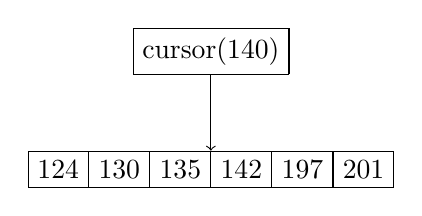
\begin{tikzpicture}
        \tikzstyle{bplus}=[rectangle split, rectangle split horizontal,rectangle
        split ignore empty parts,draw] \tikzstyle{every node}=[bplus]
        \node {cursor(140)} [->]
        child {node[rectangle split parts=6] {124\nodepart{two} 130\nodepart{three} 135\nodepart{four} 142\nodepart{five} 197\nodepart{six} 201}};
      \end{tikzpicture}
    \end{center}
  \end{itemize}
\item<4-> However, it can be anything that implements the interface
  functions
  \begin{itemize}
  \item A stupid one could simply save the key in the cursor 
  \end{itemize}
\end{itemize}

\end{frame}

\begin{frame}[t,fragile]
\frametitle{Interface of Cursored Table}

\begin{onlyenv}<1>
  \begin{block}{Specification for a Cursored Table}
    \begin{minted}[fontsize=\footnotesize]{coq}
Module Type CursoredTable (K: OrderedType).
  Parameter table: Type -> Type.
  Parameter cursor: Type -> Type.
  Section Types.
    Variable elt: Type.
    Parameter make_cursor: K.t -> table elt -> cursor elt.
    Parameter get: cursor elt -> table elt -> option (K.t * elt).
    Parameter put: cursor elt -> elt -> table elt ->
                   (cursor elt * table elt).
  End Types.
End Table.
    \end{minted}
  \end{block}
\end{onlyenv}

\begin{onlyenv}<2>
  \begin{block}{Specification for a Cursored Table(Count.)}
    \begin{minted}[fontsize=\footnotesize]{coq}
Module Type CursoredTable (K: OrderedType).
  Parameter table: Type -> Type.
  Parameter cursor: Type -> Type.
  Section Types.
    [...]
    Parameter next_cursor: cursor elt -> table elt -> cursor elt.
    Parameter prev_cursor: cursor elt -> table elt -> cursor elt.
    Parameter first_cursor: table elt -> cursor elt.
    Parameter last_cursor: table elt -> cursor elt.
  End Types.
End Table.
    \end{minted}
  \end{block}
\end{onlyenv}

\begin{onlyenv}<3>
  \begin{block}{Specification for a Cursored Table(Count.)}
    \begin{minted}[fontsize=\footnotesize]{coq}
Module Type CursoredTable (K: OrderedType).
  Parameter table: Type -> Type.
  Parameter cursor: Type -> Type.
  Section Types.
    [...]
    Parameter table_correct: table elt -> Prop.
    Parameter cursor_correct: table elt -> Prop.
    Parameter abs_rel: cursor elt -> table elt -> Prop.
    Parameter key_rel: K.t -> cursor elt -> table elt -> Prop.
    Parameter eq_cursor: cursor elt -> cursor elt ->
                         table elt -> Prop.
  End Types.
End Table.
    \end{minted}
  \end{block}
\end{onlyenv}

\begin{onlyenv}<4>
  \begin{block}{Specification for a Cursored Table(Count.)}
    \begin{minted}[fontsize=\footnotesize]{coq}
Module Type CursoredTable (K: OrderedType).
  Parameter table: Type -> Type.
  Parameter cursor: Type -> Type.
  Section Specs.
    [...]
    Axiom make_cursor_key:
      table_correct t -> key_rel k (make_cursor k t) t.
    Axiom put_shadow:
      key_rel k c1 (snd (put k e c2 t)) ->
      key_rel k c2 t ->
      get c1 (snd (put k e c2 t)) = Some (k, e).
  End Specs.
End Table.
    \end{minted}
  \end{block}
\end{onlyenv}


\begin{onlyenv}<5>
  \begin{block}{Specification for a Cursored Table(Count.)}
    \begin{minted}[fontsize=\footnotesize]{coq}
Module Type CursoredTable (K: OrderedType).
  Parameter table: Type -> Type.
  Parameter cursor: Type -> Type.
  Section Specs.
    [...]
    Axiom next_order:
      ~ eq_cursor c (last_cursor t) t ->
      key_rel k1 c t -> key_rel k2 (next_cursor c t) t ->
      KeyType.lt k1 k2.
    Axiom next_compact:
      ~ eq_cursor c (last_cursor t) t ->
      key_rel k1 c t -> key_rel k2 (next_cursor c t) t ->
      forall c' k3,
      ~ eq_cursor c c' t -> key_rel k3 c' t ->
      lt k3 k1 \/ gt k3 k2.
  End Specs.
End Table.
    \end{minted}
  \end{block}
\end{onlyenv}

% TODO:

\end{frame}

\section{Table with Flattening}

\begin{frame}[t,fragile]
\frametitle{A Functional Client's Perspective}

Suppose we are going to define a tree with finite degrees. \\

\begin{onlyenv}<2>
  \begin{block}{Tradition Definition}
\begin{minted}[fontsize=\footnotesize]{coq}
Inductive tree: Type :=
| node_of: list tree -> tree.
\end{minted}
  \end{block}
\end{onlyenv}

\only<3->{Now suppose we have a key associated with each subtree.}

\begin{onlyenv}<4->
  \begin{alertblock}{Definition as a Client of Table}
\begin{minted}[fontsize=\footnotesize]{coq}
Module Tree (K: DecidableType) (NodeTable: Table K).
  Inductive tree: Type :=
  | node_of: NodeTable.table tree -> tree.
End Tree.
\end{minted}
  \end{alertblock}
\end{onlyenv}

\only<5->{This doesn't work! Coq has no knowledge about positiveness about
  \texttt{NodeTable.table}.}

\end{frame}

\begin{frame}
\frametitle{Remedy for the Problem}

To make the module type useful for such a client, there are possible several
solutions.

\begin{itemize}
\item<2-> Turn off the positive check
  \begin{itemize}
  \item<3-> not the ideal solution
  \end{itemize}
\item<4-> Define the strict-positiveness as part of the spec., and
  let the implementation prove it
  \begin{itemize}
  \item<5-> seems to be too much difficulty for an undergrad
  \end{itemize}
\item<6-> Define \texttt{flatten} function that turns the table into some
  already known strict positive type
  \begin{itemize}
  \item<7-> our choice!
  \end{itemize}
\end{itemize}

\end{frame}

\begin{frame}[t,fragile]
\frametitle{Choice of Flattened Form}

There are two candidates for the flatten target, either a partial function or a
list of pairs.

\begin{onlyenv}<2-4>
  \begin{block}{Definition for Some Toy Tree}
\begin{minted}[fontsize=\footnotesize]{coq}
Inductive tree: Type := node_of: Z -> (Z -> option tree) -> tree.
\end{minted}
  \end{block}
\end{onlyenv}

\begin{onlyenv}<3-4>
  \begin{alertblock}{Representation Predicate for Partial Function Form}
\begin{minted}[fontsize=\footnotesize]{coq}
Fixpoint tree_rep {cs: compspecs} (k: Z) (t: tree): mpred :=
  match t with
  | node_of n subtrees =>
    EX p: val, data_at Tsh tint (Vint (Int.repr n)) p *
    (ALL k': Z, ALL t': tree,
     !! (subtrees k' = Some t') -* (tree_rep k' t'))
  end.
\end{minted}
  \end{alertblock}
\end{onlyenv}

\only<4>{It turns out we need to \textit{flatten} the partial function again
  into a list to make it work.}

\begin{onlyenv}<5-6>
  \begin{block}{Definition for Some Toy Tree}
\begin{minted}[fontsize=\footnotesize]{coq}
Inductive tree: Type := node_of: Z -> list (Z * tree) -> tree.
\end{minted}
  \end{block}
\end{onlyenv}

\begin{onlyenv}<6>
  \begin{block}{Representation Predicate for List Form}
\begin{minted}[fontsize=\footnotesize]{coq}
Fixpoint tree_rep {cs: compspecs} (k: Z) (t: tree): mpred :=
  match t with
  | node_of n subtrees =>
    EX p: val, data_at Tsh tint (Vint (Int.repr n)) p *
    iter_sepcon (fun b => tree_rep (fst b) (snd b)) subtrees
  end.
\end{minted}
  \end{block}
\end{onlyenv}

\end{frame}

\begin{frame}[t, fragile]
\frametitle{Strengthen the Flattening}

Guaranteeing the shape of flattened table is not satisfiable for the client,
because all the beautiful properties of the table are lost. \\ \pause

It would be great if the flattened list still provides \texttt{get} and
\texttt{put} functions and certain properties. \pause

\begin{onlyenv}<3>
  \begin{block}{List Table}
\begin{minted}[fontsize=\footnotesize]{coq}
Module ListTable (K: DecidableType) <: Table K.
  Definition table (elt: Type): Type := list (K.t * elt).
  [...]
End Module.
\end{minted}
  \end{block}
\end{onlyenv}

\begin{onlyenv}<4>
  \begin{block}{Flattenable Table}
\begin{minted}[fontsize=\footnotesize]{coq}
Module Type FlattenableTable (K: DecidableType) <: Table K.
  Include Table K.
  Module Flattened := ListTable K.t.
  Section Types.
    Variable elt: Type.
    Parameter flatten: table elt -> Flattened.table elt.
  End Types. 
End Module.
\end{minted}
  \end{block}
\end{onlyenv}

\begin{onlyenv}<5>
  \begin{block}{Flattenable Table(Count.)}
\begin{minted}[fontsize=\footnotesize]{coq}
Module Type FlattenableTable (K: DecidableType) <: Table K.
  [...]
  Section Specs.
    Axiom flatten_correct: forall t,
      table_correct t ->
      Flattened.table_correct (flatten t) /\
      forall (k: K.t), get k t = Flattened.get k (flatten t).
  End Specs. 
End Module.
\end{minted}
  \end{block}
\end{onlyenv}

\begin{onlyenv}<6>
  \begin{block}{Some Useful Flattenable Table Facts}
\begin{minted}[fontsize=\footnotesize]{coq}
Module FlattenableTableFacts
   (K: DecidableType) (T: FlattenableTable K).
  Include T.
  [...]
  Theorem put_permute (k: key) (v: elt) (t: table elt):
    table_correct t ->
    flatten (put k v t) = put k v (flatten t). 
End Module.
\end{minted}
  \end{block}
\end{onlyenv}

\end{frame}

\begin{frame}
\frametitle{Extending Flattening to Cursored Table}

It turns out, the \texttt{flatten} can be extended to table with cursors as
well. \\ \pause

Of course, there is much more effort when proving with cursors.

\end{frame}

\section{Progress and the Future}

\begin{frame}
\frametitle{What Are Done So Far}

\begin{itemize}
\item<1-> We have a relatively complete spec. for the cursored tables (Brian
  and Luke)
\item<2-> We have verified the implementation of B+-Trees in C with respects to
  the functional implementation (Aurele)
\item<3-> An cursored table implemented by sorted list and related facts have
  been (mostly) proven for clients
\end{itemize}

\end{frame}

\begin{frame}
\frametitle{What Will be in the Future}

\begin{itemize}
\item An ongoing effort to verify a trie as both an client and provider of
  this spec.
  \begin{itemize}
  \item As a verification of the correctness of the spec.
  \end{itemize}
  \pause
\item DeepSpecDB will be using the spec. as the index engine for the
  relational database
\end{itemize}

\end{frame}

\begin{frame}
  \begin{center}
    \Large{Thanks!}
  \end{center}

\end{frame}

\end{document}
